\documentclass[a4paper]{article}


\usepackage[russian]{babel}
\usepackage[utf8]{inputenc}
\usepackage{graphicx}


\title{Лабораторная работа №2}
\author{Антипов Денис, гр. 5539 (вариант 17 (1))}

\begin{document}
\maketitle

\section{Описание задачи}

Разработать real-coded алгоритм, минимизирующий на квадрате $-5.12 \le x, y \le 5.12$ функцию
$$f(x, y) = x^2 + y^2.$$

\section{Описани алгоритма}
\begin{itemize}
\item Варьируемые параметры алгоритма:
\begin{itemize}
\item Турнирная вероятность
\item Вероятность кроссинговера
\item Вероятность мутации
\item Коэффициент расширения кроссинговера
\item Размер популяции
\item Размер следующего поколения
\end{itemize}
\item Индивид представляется вектором с двумя вещественными координатами. Первое поколение генерируется случайно, все индивиды равномерно распределены по квадрату, в котором происходит поиск.
\item Оператор редукции использует турнирный отбор для выбора двух родителей. Оператор аналогичен описанному подробно в моем отчете к ЛР №1
\item Далее используется опреатор линейного расширенного кроссинговера с вероятностью кроссинговер. При этом коэффициент расширения может настраиваться перед запуском расширения.
\item Оператор мутации случайным образом изменяет одну из координат каждого индивида из нового поколения с вероятностью мутации.
\item Новое поколение доукомплектовываается до размера популяции лучшими особями прошлого поколения.
\end{itemize}

\section{Результаты работы алгоритма}

Результат одного из запусков алгоритма показан на рисунках ниже: 

\begin{tabular}{c}
Начальное распределение \\
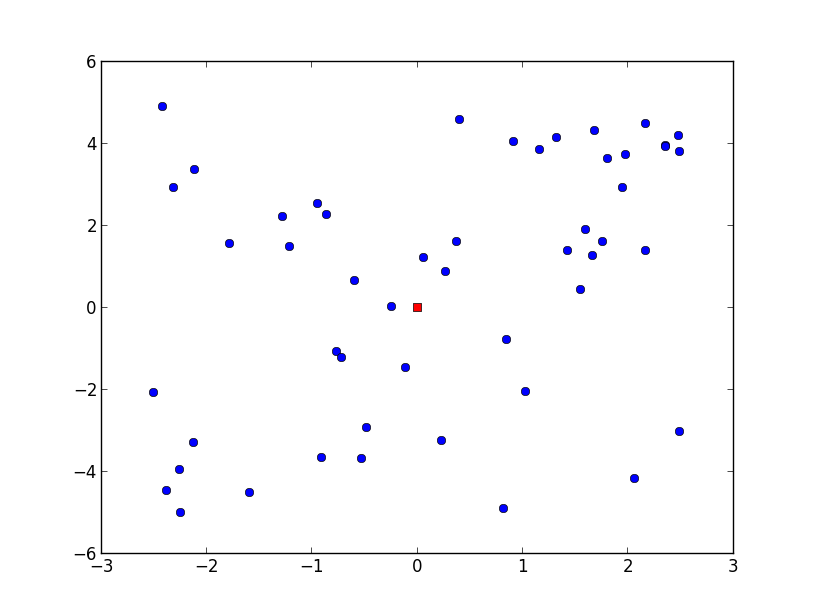
\includegraphics[width=12cm]{start.png} \\
Конечное распределение  \\
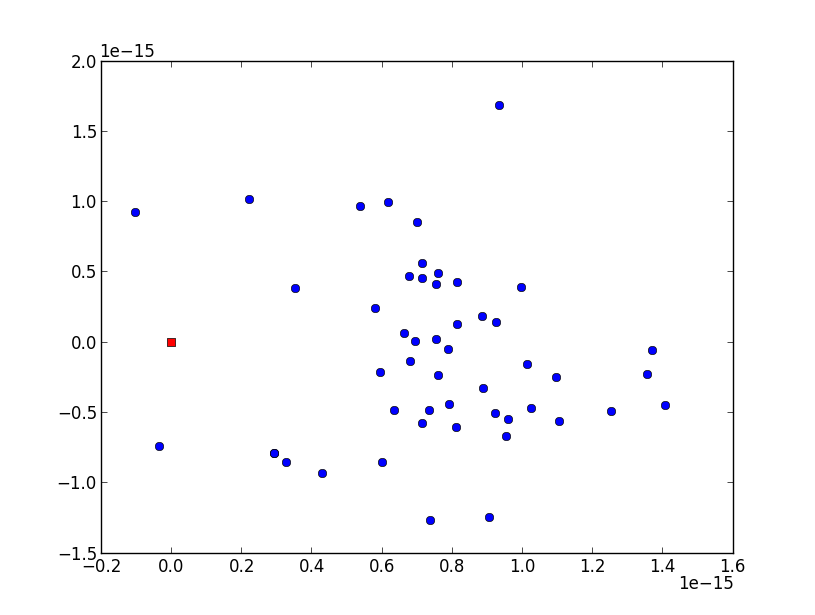
\includegraphics[width=12cm]{end.png}
\end{tabular}

Наилучшя точка: $f(3.53 \cdot 10^{-16}, 3.83 \cdot 10^{-16}) = 2.71 \cdot 10^{-31}$

В этом запуске, как и в других, алгоритм не нашел точного оптимума, но нашел достаточно точный результат.

Варьирование параметров давало следующие результаты:
\begin{itemize}
\item Уменьшение турнирной вероятности, вероятности кроссинговера и размера следующего поколения относительно размера популяции уменьшали скорость сходимости алгоритма.
\item Изменение вероятности мутации почти не влияло на сходимость алгоритма, разве что в конечном результате иногда появлялись точки, начительно отдаленные от оптимума.
\item Уменьшение коэффициента расширения в кроссинговере приводило к сходимости точек дальше от реального оптимума, что понижало точность. Такое случалось, когда все особи популяции имель одну координату строго больше или строго меньше одной из координат оптимума.
\end{itemize}
\end{document}